% Section content template for individual Educative lessons
% This file contains the actual content for a specific section
% Generated from Educative API section content

% Section: Sequence Diagram for Stack Overflow
% Section ID: 5490623111233536
% Section Slug: sequence-diagram-for-stack-overflow
% Generated: 2025-12-12T22:50:20.013194

Sequence diagrams are a great way to understand the interactions between different entities and objects in the system. There can be different sequence diagrams that we can create for Stack Overflow. In this lesson, we will create sequence diagrams for the following two interactions:

\begin{itemize}
\item
\protect\phantomsection\label{wUElxVdZvWzYsiOqk_15C}
\textbf{Close question:} A user votes to close a question authored by a different user.
\item
\protect\phantomsection\label{ip5KPpK-MsuRETat0_vdb}
\textbf{Sequence challenge:} A user creates a question and adds a bounty.
\end{itemize}

\subsection{Close question}\label{cjErOWWT4x6R7sXauyPW2}
\\
The sequence diagram for closing a question should have the following actors and objects that will interact with each other:

\begin{itemize}
\item
\protect\phantomsection\label{ypniRu1d3KSzX-oQQjdB-}
\textbf{Actors:} \texttt{User} and \texttt{Author}
\item
\protect\phantomsection\label{sCfb4BbleY_RknEvLc47a}
\textbf{Object:} \texttt{Question}
\end{itemize}
\\
Here are the steps in the closed-question interaction:

\begin{enumerate}
\item
\protect\phantomsection\label{CqAp58X54x-6zeDsfBdl5}
A user votes to close a question with some remark.
\item
\protect\phantomsection\label{D63G0q7YgiTqTqRidLQt2}
If the user is a moderator:

\begin{enumerate}
\item
The question is closed.
\item
The author of the question is notified about the question.
\end{enumerate}
\item
\protect\phantomsection\label{_gajBKb5AUtwqU7_JV2iC}
Else if they are a regular user:

\begin{enumerate}
\item
If the user's reputation is greater than or equal to 3000:

\begin{enumerate}
\item
A close vote is added.
\item
If there are 3 close votes, the question closes, and the author is notified.
\end{enumerate}
\item
Else if the user's reputation is less than 3000:

\begin{enumerate}
\item
The vote is considered invalid.
\end{enumerate}
\end{enumerate}
\end{enumerate}
\\
Based on the order above, the sequence diagram for closing a question in Stack Overflow is provided below:

\begin{figure}[htbp]
 \centering
 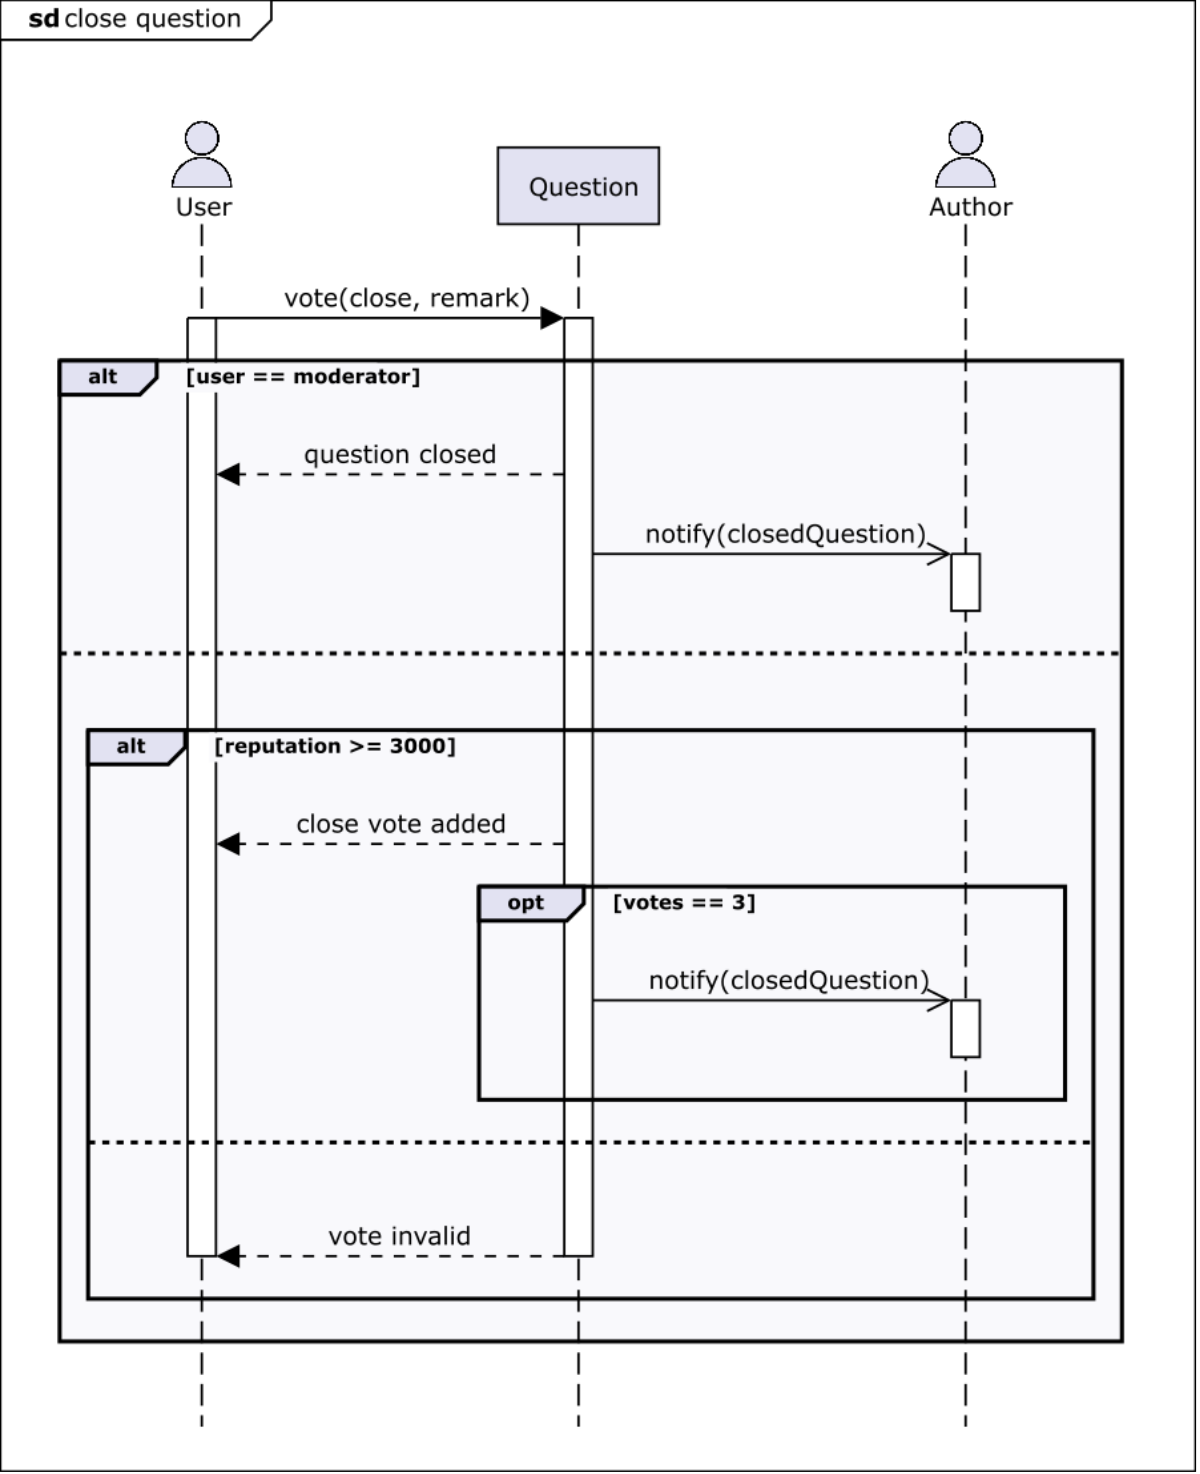
\includegraphics[width=0.5\textwidth]{Images/chapter_20/section_5490623111233536/6363272166244352.png}
 \caption{The sequence diagram for closing a question}
\end{figure}

\subsection{Sequence challenge: Create question}\label{7HH-ohlZCL_AzGGi90cbS}
\\
You'll help us complete a sequence diagram for a new question created by a user where the user adds a bounty to the question after publishing it. A skeleton of the create question sequence diagram is given below:

\begin{figure}[htbp]
 \centering
 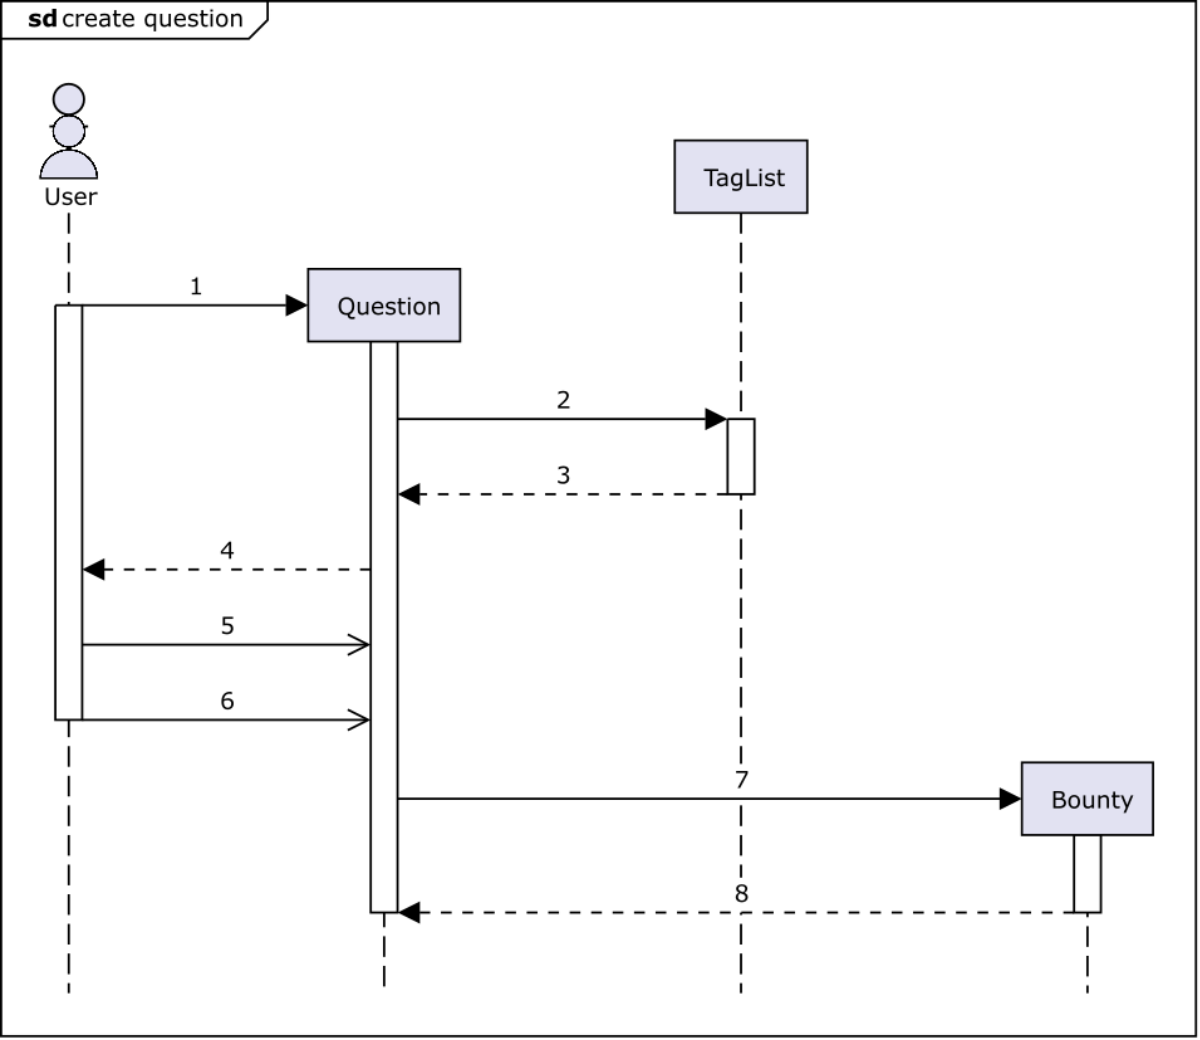
\includegraphics[width=0.5\textwidth]{Images/chapter_20/section_5490623111233536/5662620843769856.png}
 \caption{The sequence diagram for creating a question}
\end{figure}

Notice that the arrows in the diagram above are numbered from 1 to 8. Below are the messages between the actor(s) and object(s). Can you rearrange the messages below in the correct order sequence they should appear in the skeleton of the sequence diagram provided above?
\begin{quote}
\textbf{Note:} If you're stuck, click the ``Show Solution'' button.
\end{quote}

Alternatively, you can click the ``Show complete diagram'' button below to see the complete sequence diagram for creating a question interaction.

Next, let's examine the activity diagrams for Stack Overflow to understand the system's control flow.

% End of section content